\section{Versuchsbeschreibug}
\label{section:Versuchsbeschreibung}
Beschreiben Sie kurz in zusammenhängenden Sätzen den Versuchsaufbau. Notwendig ist auch eine Skizze mit allen genutzten Messpunkten. Genutzte Abbildungen bekommen grundsätzlich eine Bildunterschrift und werden ebenfalls fortlaufend nummeriert (siehe \fref{BspVers}).\\

%
\begin{figure}[!h]
		\centering
		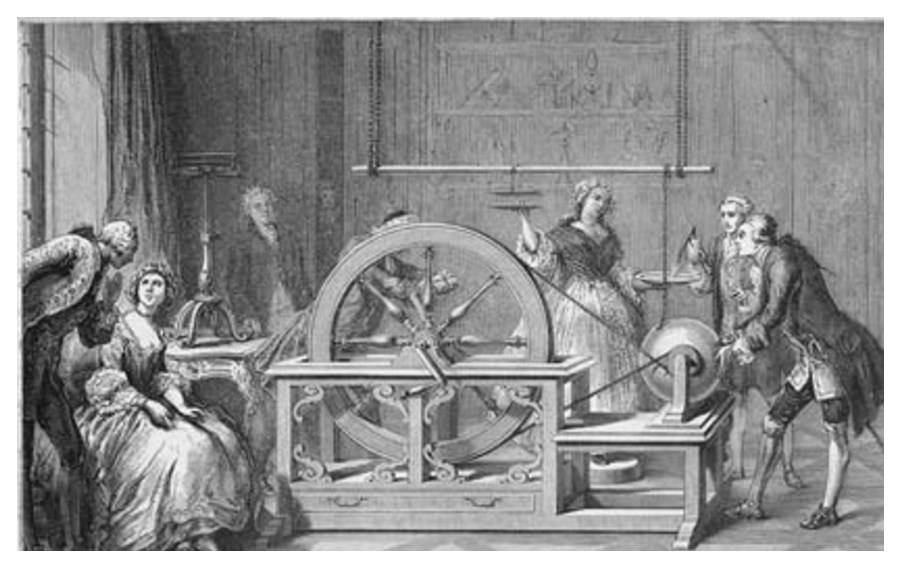
\includegraphics[width=0.5\textwidth]{Abbildungen/Beispielbild_Versuchsaufbau.eps}
		\caption{Foto oder Skizze des Versuchsaufbaus}
		\label{fig:BspVers}
\end{figure}
%
Werden Textpassagen (wie z.B. Definitionen) wörtlich übernommen, dann müssen diese auch durch eine Quellenangabe kenntlich gemacht werden. Die dazugehörigen Quellen werden im Literaturverzeichnis aufgeführt.\\

Die verwendeten Messgeräte und deren Genauigkeit sind als Auflistung oder tabellarisch darzustellen.\\

Beispiel:
%
\begin{itemize}
\item Laser-Umdrehungsmesser Conrad DT2234C, Auflösung 1 1/min $\pm$1 Digit
\end{itemize}
%
